\documentclass[11pt]{article}
\usepackage[margin=2.3cm]{geometry}
\usepackage{amsmath,amssymb}
\usepackage{graphicx}
\usepackage{booktabs}
\usepackage{array}
\usepackage{float}
\usepackage{caption}
\usepackage[hidelinks]{hyperref}
\captionsetup{font=small,labelfont=bf}
\graphicspath{{figs/}}
\newcommand{\code}[1]{\texttt{#1}}
\newcommand{\sig}{\boldsymbol\sigma}

\title{Duvaut--Lions viscoplastic regularization in DynEarthSol:\\
formulation, mesh convergence, choice of $\tau$ and the mesh, and limitations}
\author{}
\date{November 2026}

\begin{document}
\maketitle

\begin{abstract}
With rate-independent, strain-softening Mohr--Coulomb plasticity, the shear bands of DynEarthSol
(DES) have no length scale of their own: their width is a few elements and halves when the mesh is
refined. Branch \code{feat/regularization} adds a Duvaut--Lions regularization
(\code{control.has\_duvaut\_lions}, \code{mat.relaxation\_time}~$\tau$) that lets the stress exceed
the yield surface by an overstress that relaxes over $\tau$. This makes the plastic flow rate
dependent, with a viscoplastic viscosity $\eta_{vp}=G\tau$, and gives the band a physical width
$W\sim G\tau V/\Delta c$ set by $\tau$, the slip rate $V$ and the strength lost by softening
$\Delta c$. On the core-complex example the main-fault width becomes mesh independent
(1.34 and 1.35\,km at 250 and 167\,m for $\tau=3.3\times10^8$\,s) once about five elements span it.
This note explains the formulation and why it works, documents the convergence study (issue \#109),
gives the recipe for choosing $\tau$ and the mesh, shows that it combines with high-pass mass damping
without changing the regularized fault while the damping removes the noise that remains, and lists
the limitations: the resolution
requirement, its interplay with seeds and refined zones, the overstress it adds to fault strength,
and what has not been tested.
\end{abstract}

\tableofcontents

%======================================================================
\section{The problem: softening bands follow the mesh}
\label{sec:problem}

In \code{rh\_ep} (and the plastic part of \code{rh\_evp}) DES uses a rate-independent
Mohr--Coulomb return map: if the elastic trial stress lies outside the yield surface it is returned
onto it within the step, and the cohesion (and friction) soften linearly with the accumulated
plastic strain $\kappa$ from \code{cohesion0} at $\kappa=$\,\code{pls0} to \code{cohesion1} at
\code{pls1}.

Softening makes the localization problem ill posed: nothing in the equations prefers a band of one
width over another, so the band narrows until the discretization stops it --- at a few elements.
Table~\ref{tab:conv} (``original code'') shows it on the core-complex example: the main fault is
1.33\,km wide at 500\,m, 0.64\,km at 250\,m and 0.34\,km at 167\,m (15--30\,kyr), halving with the
element size. In the companion note on high-pass damping the same setup gave 1.8, 1.2 and 0.3\,km at
1000, 500 and 167\,m, with or without damping: damping removes noise but adds no length scale.
Quantities that depend on the band --- its width, the plastic-strain-rate integral, the strain
inside it --- therefore do not converge, and neither, in general, does the fault pattern (the
original code at 167\,m abandons the main fault by 50\,kyr; Fig.~\ref{fig:taumaps}).

%======================================================================
\section{Formulation}
\label{sec:form}

\subsection{The Duvaut--Lions update}
Duvaut--Lions viscoplasticity lets the stress relax towards the rate-independent solution
$\sig^{RI}$ over a time $\tau$ instead of reaching it instantly:
\begin{equation}
  \dot\sig = \mathbf C:\dot{\boldsymbol\varepsilon} - \frac{\sig-\sig^{RI}}{\tau}.
\end{equation}
Integrated with backward Euler over a step $\Delta t$, starting from the elastic trial stress
$\sig^{tr}=\sig_n+\mathbf C:\Delta\boldsymbol\varepsilon$, this gives a weighted mean of the trial
stress and the ordinary return-mapped stress:
\begin{equation}
  \sig_{n+1} = (1-w)\,\sig^{tr} + w\,\sig^{RI},\qquad
  \Delta\kappa = w\,\Delta\kappa^{RI},\qquad
  w = \frac{\Delta t}{\tau+\Delta t}.
  \label{eq:dl}
\end{equation}
The plastic-strain increment is scaled by the same $w$, so softening advances at the regularized
rate. $\tau=0$ gives $w=1$, the rate-independent return, bit for bit.

\subsection{Implementation}
A single helper, \code{plastic\_candidate()} in \code{rheology.cxx}, computes the elastic trial
(the same one \code{elasto\_plastic\{,2d\}()} start from, including plane strain and
effective-stress variants), calls the unchanged return map, and blends the two by $w$. It serves
\code{rh\_ep} and the plastic candidate of \code{rh\_evp}; the Maxwell (viscous) candidate of
\code{rh\_evp} is untouched, and \code{rh\_evp} still keeps whichever candidate has the smaller
second invariant. Options:
\begin{itemize}
\item \code{control.has\_duvaut\_lions} (default \emph{no});
\item \code{mat.relaxation\_time} $=[\tau_0,\tau_1,\dots]$, per material, in seconds (default
  $[0]$); $\tau=\eta_{vp}/G$ relates it to a viscoplastic viscosity.
\end{itemize}
Other rheologies (\code{elastic}, \code{viscous}, \code{maxwell}, both rate-and-state types) and
$\tau<0$ are rejected at startup. Verification: flag off, and flag on with $\tau=0$, are
bit-identical to the parent commit on \code{test-3d-equ-tiny}, \code{test-3d-remesh},
\code{test-tiny} and \code{test-core}, plus plane-strain and \code{rh\_evp} variants of
\code{test-core}; $\tau=10^{10}$\,s changes \code{rh\_ep} and \code{rh\_evp} results in 2D, 3D and
plane strain.

\subsection{What the update does: one element}
For $\Delta t\ll\tau$, Eq.~\eqref{eq:dl} gives a plastic strain rate
$\dot\kappa\approx\Delta\kappa^{RI}/\tau$. Since $\Delta\kappa^{RI}$ is the overstress
$f=\sigma^{tr}-\sigma^{RI}$ divided by the (softened) modulus, this is
\begin{equation}
  f \approx G\tau\,\dot\kappa = \eta_{vp}\,\dot\kappa,\qquad \eta_{vp}=G\tau:
  \label{eq:over}
\end{equation}
the stress exceeds the yield strength by a viscous overstress proportional to the plastic strain
rate. Figure~\ref{fig:element} shows this on a single element loaded in shear at
$10^{-12}$\,s$^{-1}$ with the core-complex properties ($G=30$\,GPa, cohesion softening from 44 to
4\,MPa over $\kappa=0.5$, $\Delta t=5.6\times10^4$\,s). The rate-independent element yields at
44\,MPa and follows the softening curve; the regularized ones run above it by
$G\tau\dot\kappa=0.9$, 3 and 10\,MPa. Panel C shows the other consequence: when the strength drops
suddenly, the rate-independent stress drops within one step, while the regularized stress relaxes
over $\tau$ (1, 3 and 10 years here). In an explicit, mass-scaled solver a one-step stress drop is
what radiates pseudo-elastic waves; the regularization spreads it over $\tau/\Delta t$ steps
($\approx6000$ at 167\,m for $\tau=3.3\times10^8$\,s).

\begin{figure}[t]
  \centering
  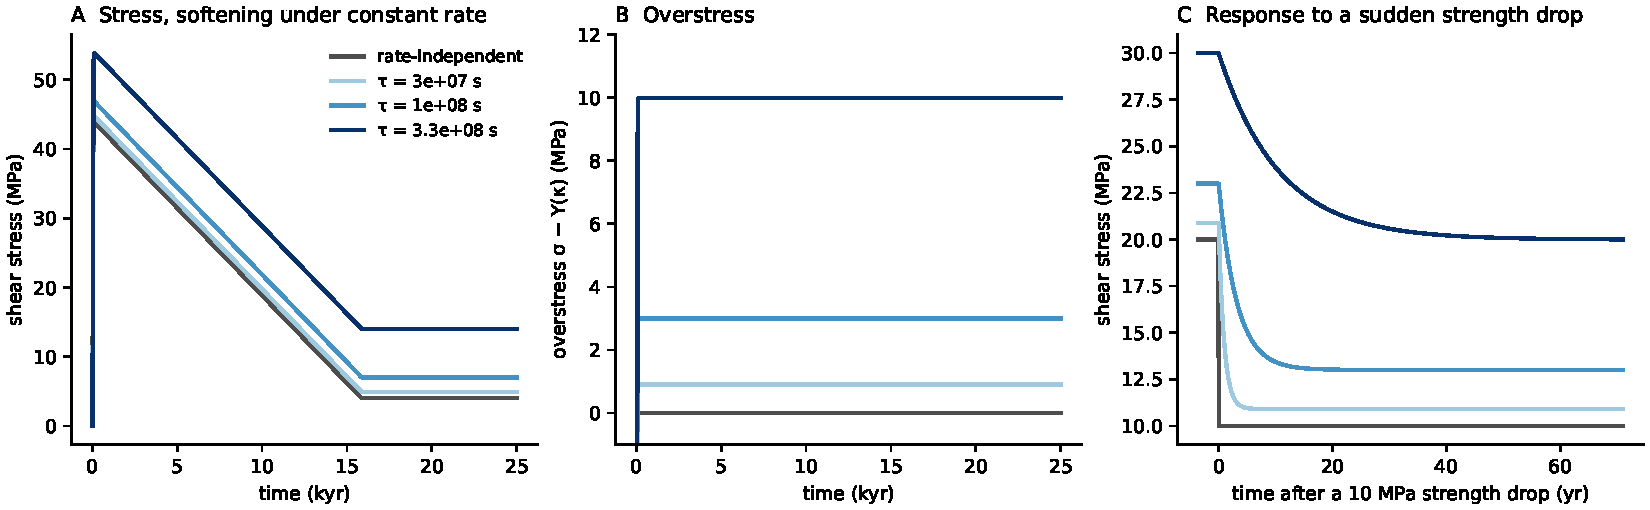
\includegraphics[width=\textwidth]{element.pdf}
  \caption{One element in shear, core-complex properties, DES-like time step. Grey:
  rate-independent; blue shades: Duvaut--Lions with $\tau=3\times10^7$, $10^8$, $3.3\times10^8$\,s.
  \textbf{A}: stress under a constant shear strain rate of $10^{-12}$\,s$^{-1}$; cohesion softens
  from 44 to 4\,MPa as $\kappa$ goes from 0 to 0.5 (16\,kyr here). \textbf{B}: the overstress above
  the current strength, $G\tau\dot\kappa$ = 0.9, 3 and 10\,MPa. \textbf{C}: a fully softened
  element flowing steadily at 20\,MPa strength (plus overstress) whose strength drops by 10\,MPa at
  $t=0$: the rate-independent stress drops in one step; the regularized stress relaxes
  exponentially over $\tau$ and keeps its overstress.}
  \label{fig:element}
\end{figure}

\subsection{Why it gives the band a width}\label{sec:width}
In a band of width $W_\perp$ (measured across it) carrying a slip rate $V$, the plastic strain rate
is of order $V/W_\perp$, so by Eq.~\eqref{eq:over} the band carries an overstress of order
$G\tau V/W_\perp$: the narrower the band, the stronger it is. Softening favours narrowing; the
rate strengthening opposes it. The band stops narrowing when the strengthening is comparable to the
strength the softening removes, $\Delta c$:
\begin{equation}
  W_\perp \sim \frac{G\,\tau\,V}{\Delta c}.
  \label{eq:width}
\end{equation}
For the core complex ($G=30$\,GPa, $\Delta c=40$\,MPa, $\tau=3.3\times10^8$\,s and the measured
slip rate on the main fault, $V\approx2\times10^{-9}$\,m/s, Table~\ref{tab:dlhp}) the right-hand side
is $\approx0.5$\,km, while the converged band is 1.15\,km across the fault (1.34\,km horizontally).
Eq.~\eqref{eq:width} is therefore a scaling only: its prefactor, $\approx2.3$, was measured on this
one case, and the width to quote is the measured one.

The measured overstress supports the scaling (Fig.~\ref{fig:overstress}): across all three $\tau$
and all three meshes, the overstress in the active band at 50\,kyr is $0.42\pm0.07$ times
$G\tau V/W_\perp$ computed from the measured width. The constant is below 1 because the strain rate
in the band is a fraction of $V/W_\perp$ and because of the invariant convention; what matters is
that it is the same for a 30-fold range of $G\tau V/W_\perp$.

The dynamic length often quoted for viscoplastic regularization, $c_s\tau$ (wave speed times
relaxation time), is not the relevant one here: in the mass-scaled quasi-static solver the pseudo
wave speed $c=10^{-4}$\,m/s would give 33\,km for $\tau=3.3\times10^8$\,s, larger than the faults.
The quasi-static balance of Eq.~\eqref{eq:width} is what sets the width.

\begin{figure}[t]
  \centering
  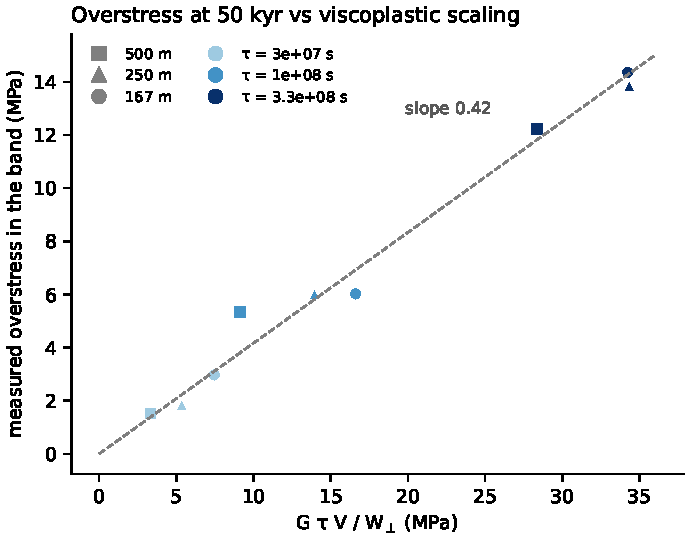
\includegraphics[width=0.55\textwidth]{overstress.pdf}
  \caption{Measured overstress in the active main-fault band at 50\,kyr against the viscoplastic
  scaling $G\tau V/W_\perp$, with $W_\perp$ the measured width (40--50\,kyr) converted to across the
  fault ($\times0.87$) and $V=4\times10^{-9}$\,m/s. Markers: mesh; shades: $\tau$. All nine runs lie
  on one line through the origin (slope 0.42; individual ratios 0.35--0.59, the largest at 500\,m
  where the band is under-resolved).}
  \label{fig:overstress}
\end{figure}

\subsection{Equivalence with a viscosity in the yield condition}
A Kelvin-type regularization that adds $\eta\dot\kappa$ to the yield function (Duretz, de Borst and
Le Pourhiet 2019, \emph{G-cubed} 20, doi:10.1029/2019GC008531) was implemented and tried on the same
setup. At $\tau=\eta/G$ it gives the same band widths within a few per cent
(Fig.~\ref{fig:methods}). Duvaut--Lions was kept because it reuses the existing return map
unchanged: the regularization is one blend after it.

%======================================================================
\section{Mesh-convergence study}
\label{sec:conv}

\paragraph{Setup.} \code{examples/core-complex.cfg} in 2D: one material, \code{pls1} = 0.5,
dilation angle 0, MMG remeshing, 50\,kyr, extension $2\times10^{-9}$\,m/s. Element sizes 500, 250 and
167\,m. $\tau=3\times10^7$, $10^8$ and $3.3\times10^8$\,s ($\eta_{vp}=9\times10^{17}$, $3\times10^{18}$,
$10^{19}$\,Pa\,s).

\paragraph{Width measure.} The horizontal width of the plastic-strain-rate band,
$\int\dot\varepsilon_p\,dx/\max\dot\varepsilon_p$, on the main fault alone, averaged over
$z=3,5,7$\,km. Across the fault (dip $\approx60^\circ$) the width is $\approx0.87$ times this.

\subsection{Two parts of the setup that had to be fixed first}
\paragraph{The seed.} The example's weak zone is 2.4\,km wide and starts fully softened
(\code{weakzone\_plstrain} = \code{pls1}). With it the regularized band simply took the seed's width:
2.05 and 2.02\,km at 500 and 250\,m for $\tau=3.3\times10^8$\,s. With a 1.2\,km seed it became 1.86,
1.48 and 1.24\,km at 500, 250 and 167\,m --- still seed controlled. All runs below use a thin,
partly softened seed: 250\,m half-width at every mesh (\code{weakzone\_halfwidth} = 1.5 elements at
167\,m) and \code{weakzone\_plstrain} = 0.1. A regularization can only set the width of a band that
is free to choose it; a seed wider than $W$ and already weakened imposes its own.

\paragraph{The refined zone.} With fine elements only over $x=38$--58\,km, the edge of the zone
started a second, conjugate fault, and the model developed a symmetric two-fault pattern that does
not form when the zone is wider (Fig.~\ref{fig:zone}). The change in element size acts as a weak
zone. All runs below refine $x=30$--70\,km at every mesh.

\begin{figure}[H]
  \centering
  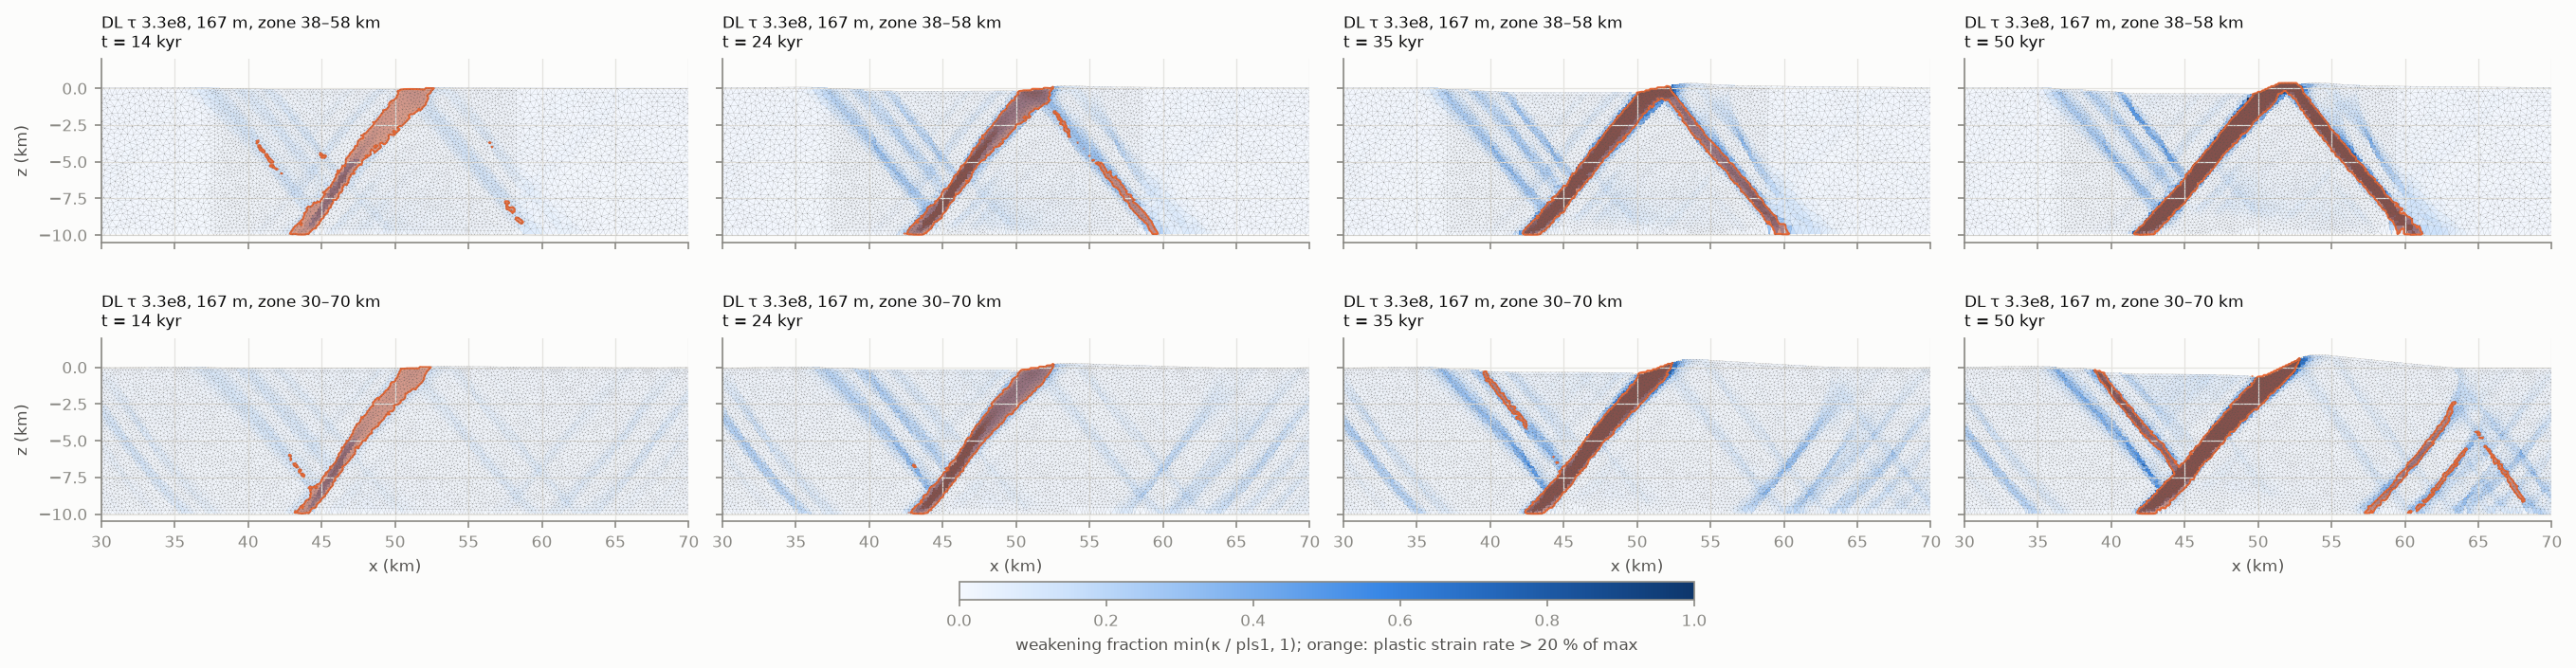
\includegraphics[width=\textwidth]{fig_zone_check.png}
  \caption{Duvaut--Lions, $\tau=3.3\times10^8$\,s, 167\,m, at 14, 24, 35 and 50\,kyr, with the
  refined zone over $x=38$--58\,km (top) and $x=30$--70\,km (bottom). Blue: weakening fraction
  $\min(\kappa/\code{pls1},1)$; orange: plastic strain rate above 20\,\% of its maximum (the active
  bands). With the narrow zone a conjugate fault starts at the zone's right edge at 24\,kyr and the
  model becomes a symmetric graben; with the wide zone one main fault carries the slip and later
  secondary faults form in the hanging wall and at $x\approx58$--68\,km.}
  \label{fig:zone}
\end{figure}

\subsection{Results}
\begin{table}[h]
  \centering\small
  \caption{Main-fault width (horizontal, km, mean of $z=3,5,7$\,km) for the thin seed and the wide
  refined zone. Last column: change from 250 to 167\,m.}
  \label{tab:conv}
  \begin{tabular}{lcccc}
  \toprule
  & 500\,m & 250\,m & 167\,m & 250$\to$167\,m\\
  \midrule
  \multicolumn{5}{l}{\emph{$t$ = 15--30\,kyr (one fault)}}\\
  original code                          & 1.33 & 0.64 & 0.34 & $-47$\,\%\\
  DL $\tau=3\times10^7$\,s               & 1.31 & 0.63 & 0.52 & $-17$\,\%\\
  DL $\tau=10^8$\,s                      & 1.32 & 0.81 & 0.72 & $-12$\,\%\\
  DL $\tau=3.3\times10^8$\,s             & 1.69 & 1.15 & 0.96 & $-16$\,\%\\
  \multicolumn{5}{l}{\emph{$t$ = 40--50\,kyr (secondary faults active)}}\\
  original code                          & 1.22 & 0.74 & 0.57 & $-23$\,\%\\
  DL $\tau=3\times10^7$\,s               & 1.24 & 0.77 & 0.55 & $-28$\,\%\\
  DL $\tau=10^8$\,s                      & 1.51 & 0.99 & 0.83 & $-16$\,\%\\
  DL $\tau=3.3\times10^8$\,s             & 1.62 & 1.34 & \textbf{1.35} & \textbf{0\,\%}\\
  \bottomrule
  \end{tabular}
\end{table}

\begin{figure}[H]
  \centering
  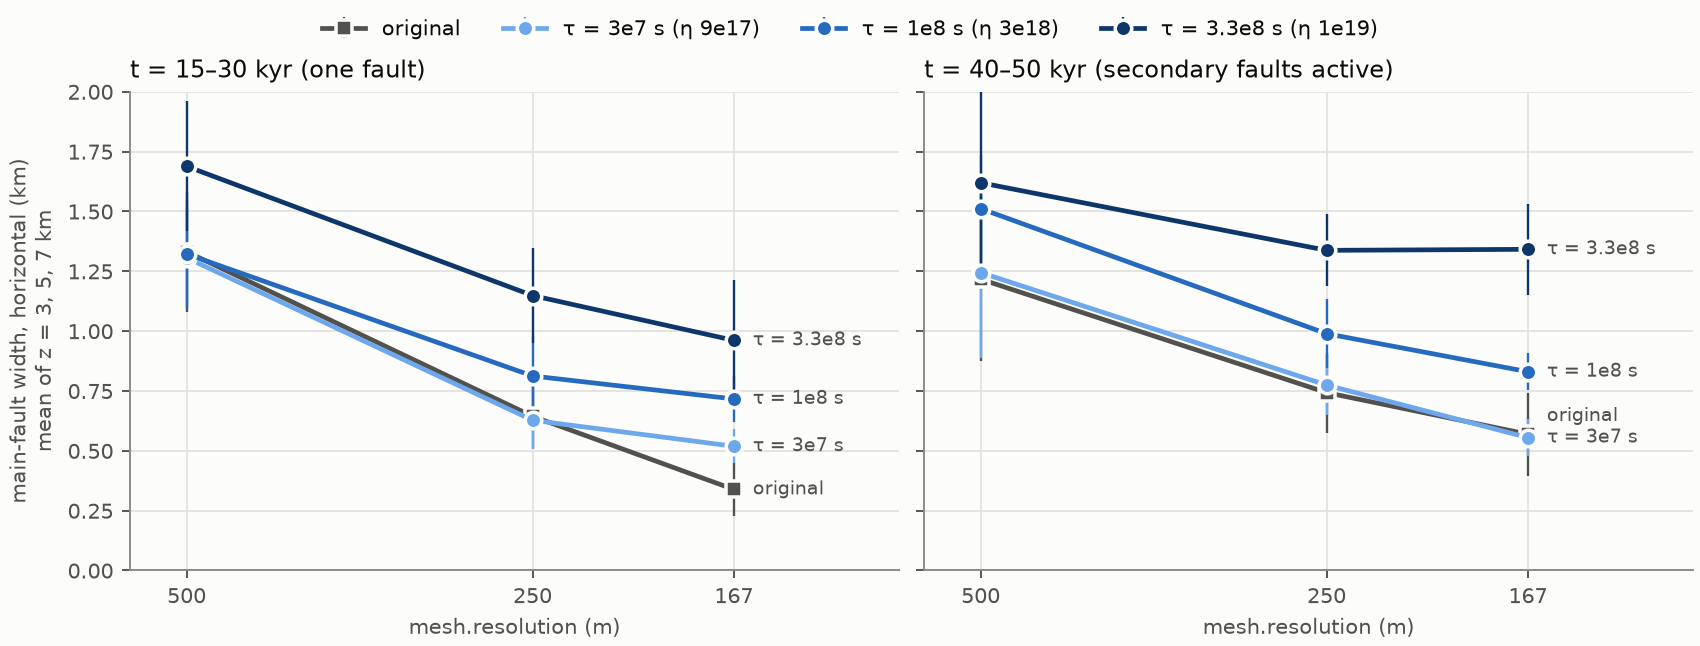
\includegraphics[width=\textwidth]{fig_main_conv.png}
  \caption{Main-fault width against element size (Table~\ref{tab:conv}); bars: standard deviation
  over the frames and depths of the window. Left: 15--30\,kyr, when one fault carries the slip.
  Right: 40--50\,kyr. The original code and $\tau=3\times10^7$\,s narrow with the mesh throughout;
  $\tau=10^8$\,s narrows less; $\tau=3.3\times10^8$\,s is flat between 250 and 167\,m late in the run.}
  \label{fig:mainconv}
\end{figure}

\begin{figure}[p]
  \centering
  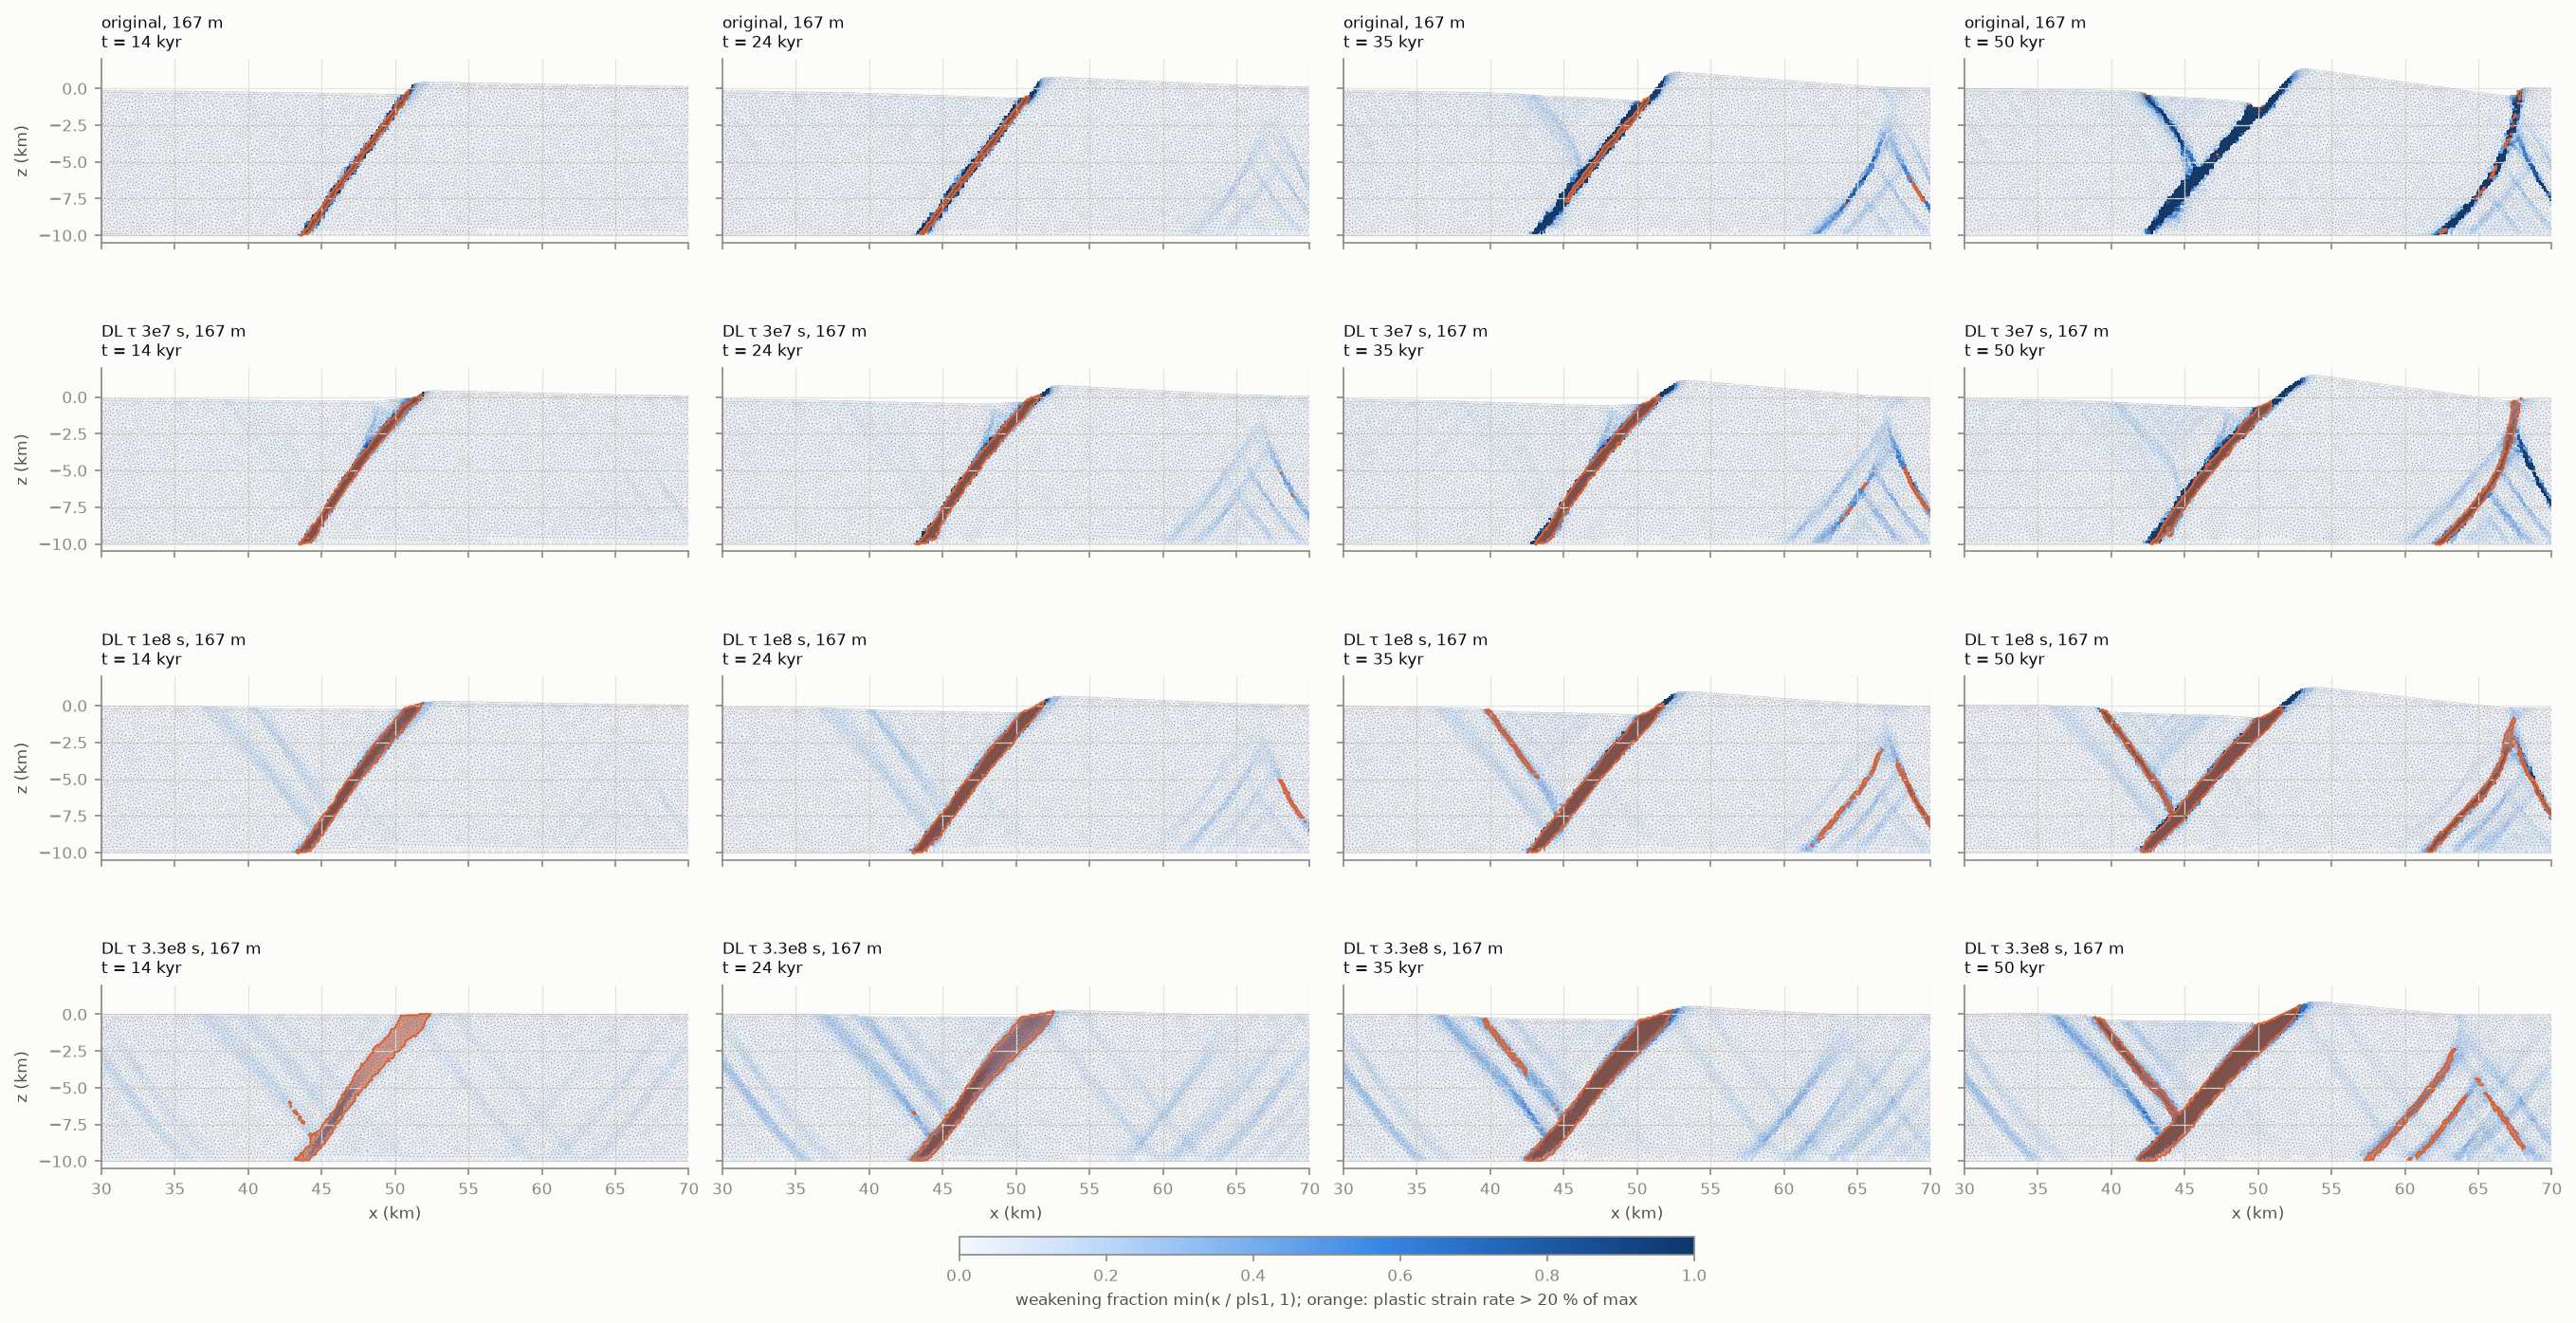
\includegraphics[width=\textwidth]{fig_tau_maps.png}
  \caption{167\,m, thin seed, wide zone, at 14, 24, 35 and 50\,kyr. Rows: original code, then
  Duvaut--Lions with $\tau=3\times10^7$, $10^8$, $3.3\times10^8$\,s. Blue: weakening fraction;
  orange: active bands (plastic strain rate above 20\,\% of maximum). The original band is one or
  two elements wide, and by 50\,kyr the main fault is mostly abandoned for faults at
  $x\approx65$\,km. The active band widens with $\tau$; at every $\tau$ one main fault carries most
  of the slip until $\sim30$\,kyr and is still the most active at 50\,kyr. With
  $\tau=3.3\times10^8$\,s the band starts wide and diffuse at 14\,kyr, narrows to its steady width
  by $\sim35$\,kyr, and secondary faults (hanging wall from $\sim35$\,kyr, $x\approx58$--68\,km near
  50\,kyr) appear.}
  \label{fig:taumaps}
\end{figure}

\paragraph{Reading the table.}
\begin{itemize}
\item \emph{Only $\tau=3.3\times10^8$\,s converges on these meshes, and only late.} Between 250 and
  167\,m its width changes by $-16$\,\% at 15--30\,kyr and 0\,\% at 40--50\,kyr, as the band widens to
  about five elements. For $\tau=10^8$\,s the change stays at $-12$ to $-16$\,\%; for
  $\tau=3\times10^7$\,s the band stays about two elements wide at 167\,m and follows the mesh. Running
  longer does not make the smaller $\tau$ converge; finer elements would.
\item \emph{The rule: count elements across the width $\tau$ sets.} A band follows the mesh when fewer
  than about three elements span the width of Eq.~\eqref{eq:width}; it is steady once about five do.
  The 500\,m mesh is too coarse for all three $\tau$.
\item \emph{The regularization keeps the core-complex geometry.} At every $\tau$ the main fault
  dominates until $\sim30$\,kyr and is still the most active at 50\,kyr. With
  $\tau=3.3\times10^8$\,s the later secondary faults appear the same way at 250 and 167\,m.
\item \emph{Overstress.} In the active band at 50\,kyr it is $\approx$2--3\,MPa for $\tau=3\times10^7$\,s,
  $\approx6$\,MPa for $10^8$\,s and $\approx$12--14\,MPa for $3.3\times10^8$\,s (up to 19\,MPa at
  35\,kyr), against a residual cohesion of 4\,MPa (Fig.~\ref{fig:overstress}).
\end{itemize}

\subsection{Comparison with other regularizations}
\begin{figure}[H]
  \centering
  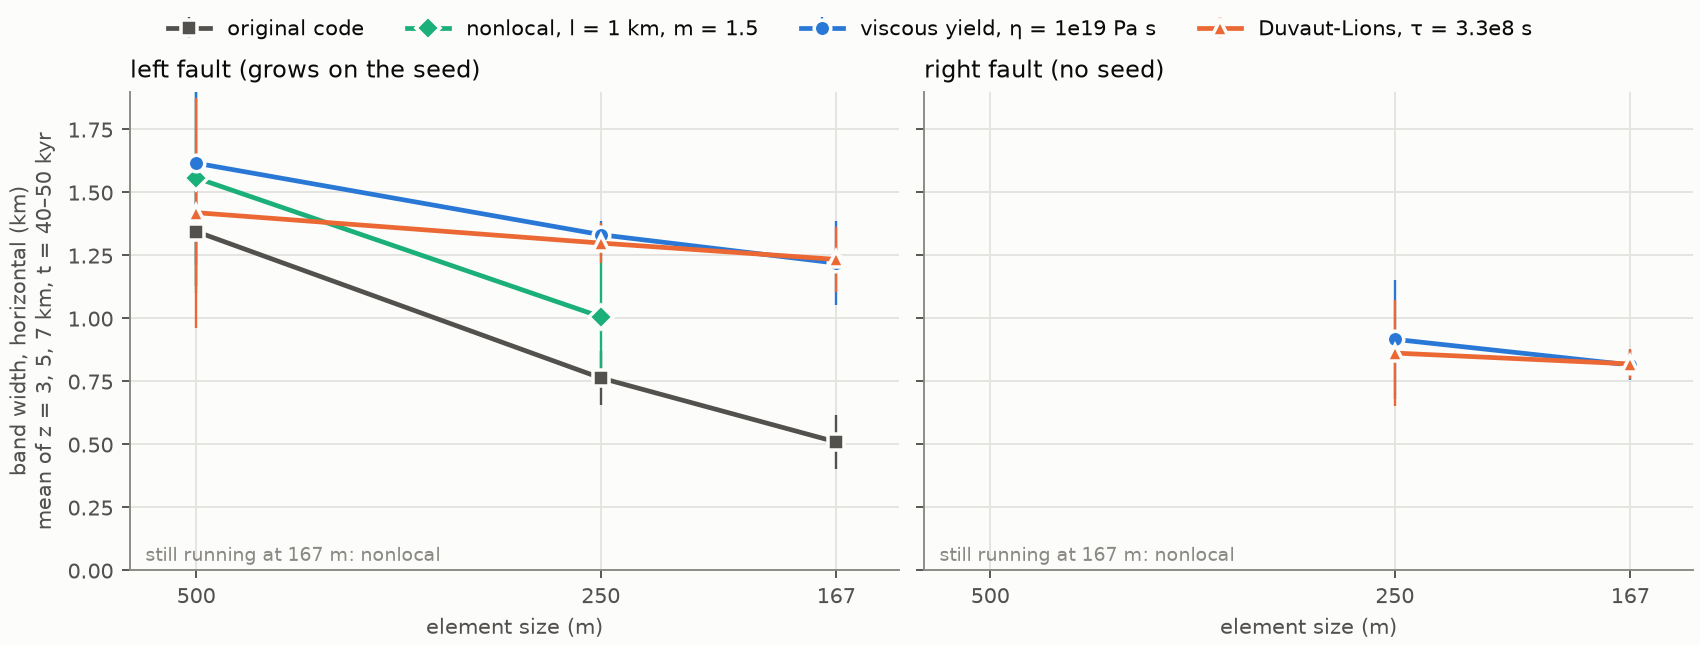
\includegraphics[width=\textwidth]{fig_thin_conv.png}
  \caption{Band width at 40--50\,kyr for four methods on the thin seed, with the \emph{narrower}
  refined zone ($x=38$--58\,km), so only trends are comparable with Table~\ref{tab:conv}. Left: the
  fault grown on the seed; right: the conjugate fault without a seed (it forms only at 250 and
  167\,m). Grey: original code; green: nonlocal averaging of the plastic-strain increment
  ($l=1$\,km, $m=1.5$; the 167\,m run did not finish); blue: viscosity in the yield condition,
  $\eta=10^{19}$\,Pa\,s; orange: Duvaut--Lions, $\tau=3.3\times10^8$\,s. The two viscoplastic
  methods agree within a few per cent and flatten with the mesh; nonlocal averaging narrows from
  1.56 to 1.01\,km (500$\to$250\,m) like the original code.}
  \label{fig:methods}
\end{figure}

Nonlocal averaging of the plastic strain (\code{mat.nonlocal\_option} = 1 on the same branch) widens
the \emph{softened} zone but does not fix the \emph{active} band: inside a converged $\sim2$\,km
softened zone the band that carries the slip still follows the mesh, and once softening saturates
($\kappa>\code{pls1}$) the nonlocal term no longer acts at all (issue \#123). The viscoplastic
regularizations act on the flow itself, at every stage.

%======================================================================
\section{Choosing $\tau$ and the mesh}
\label{sec:recipe}

\begin{enumerate}
\item \emph{Pick a target width $W$, then set} $\tau\approx W\Delta c/(2.3\,GV)$, with $\Delta c$ the
  cohesion lost by softening (\code{cohesion0} $-$ \code{cohesion1}), $G$ the shear modulus, $V$
  the expected fault slip rate and 2.3 the prefactor measured in Sect.~\ref{sec:width}.
  $\tau=3.3\times10^8$\,s gives $W=1.15$\,km for the core complex.
  Equivalently, choose a viscoplastic viscosity $\eta_{vp}=G\tau$.
\item \emph{Give every place a fault may start elements of about $W/5$}: a refined zone covering the
  weak zone from $t=0$ (\code{mesh.meshing\_option} = 2), plus MMG refinement on plastic strain
  (\code{mesh.mmg\_metric\_refine\_coeff}, e.g.\ 100) to follow faults as they grow.
\item \emph{Stop refining at $W/5$.} The metric floor is
  $\sqrt{\code{smallest\_size}}\times\code{mmg\_remesh\_defensive\_tiny\_ratio}\times\code{resolution}$.
\end{enumerate}
\code{examples/core-complex-dl.cfg} applies this for $\tau=3.333\times10^8$\,s: resolution
166.7\,m with \code{smallest\_size} = 0.23, giving a 240\,m floor ($\approx W/5$), a refined zone over
$x=41$--55\,km, $\approx570$\,m elsewhere, MMG refinement with coefficient 100, and the thin seed
(half-width 1.5 elements, \code{weakzone\_plstrain} = 0.1).

\begin{table}[h]
  \centering\small
  \caption{Main-fault width (km) for $\tau=3.3\times10^8$\,s with fixed and adaptive meshes.}
  \label{tab:amr}
  \begin{tabular}{lcccccc}
  \toprule
  mesh & 5--15 & 15--25 & 25--35 & 35--42 & 42--50\,kyr & elements\\
  \midrule
  example: 240\,m zone + MMG, floor 240\,m & 1.14 & 1.07 & 1.21 & 1.31 & 1.32 & 13\,500\\
  same, floor 160\,m                       & 1.04 & 0.92 & 1.13 & 1.19 & 1.28 & 16\,200\\
  fixed 250\,m, zone $x$ 30--70\,km         & 1.19 & 1.08 & 1.25 & 1.32 & 1.34 & 11\,200\\
  fixed 167\,m, zone $x$ 30--70\,km         & 0.94 & 0.92 & 1.08 & 1.27 & 1.35 & 25\,100\\
  500\,m + MMG refinement, coarse seed      & 1.42 & 1.28 & 1.38 & 1.39 & 1.54 & 4\,000\\
  \bottomrule
  \end{tabular}
\end{table}

\begin{figure}[p]
  \centering
  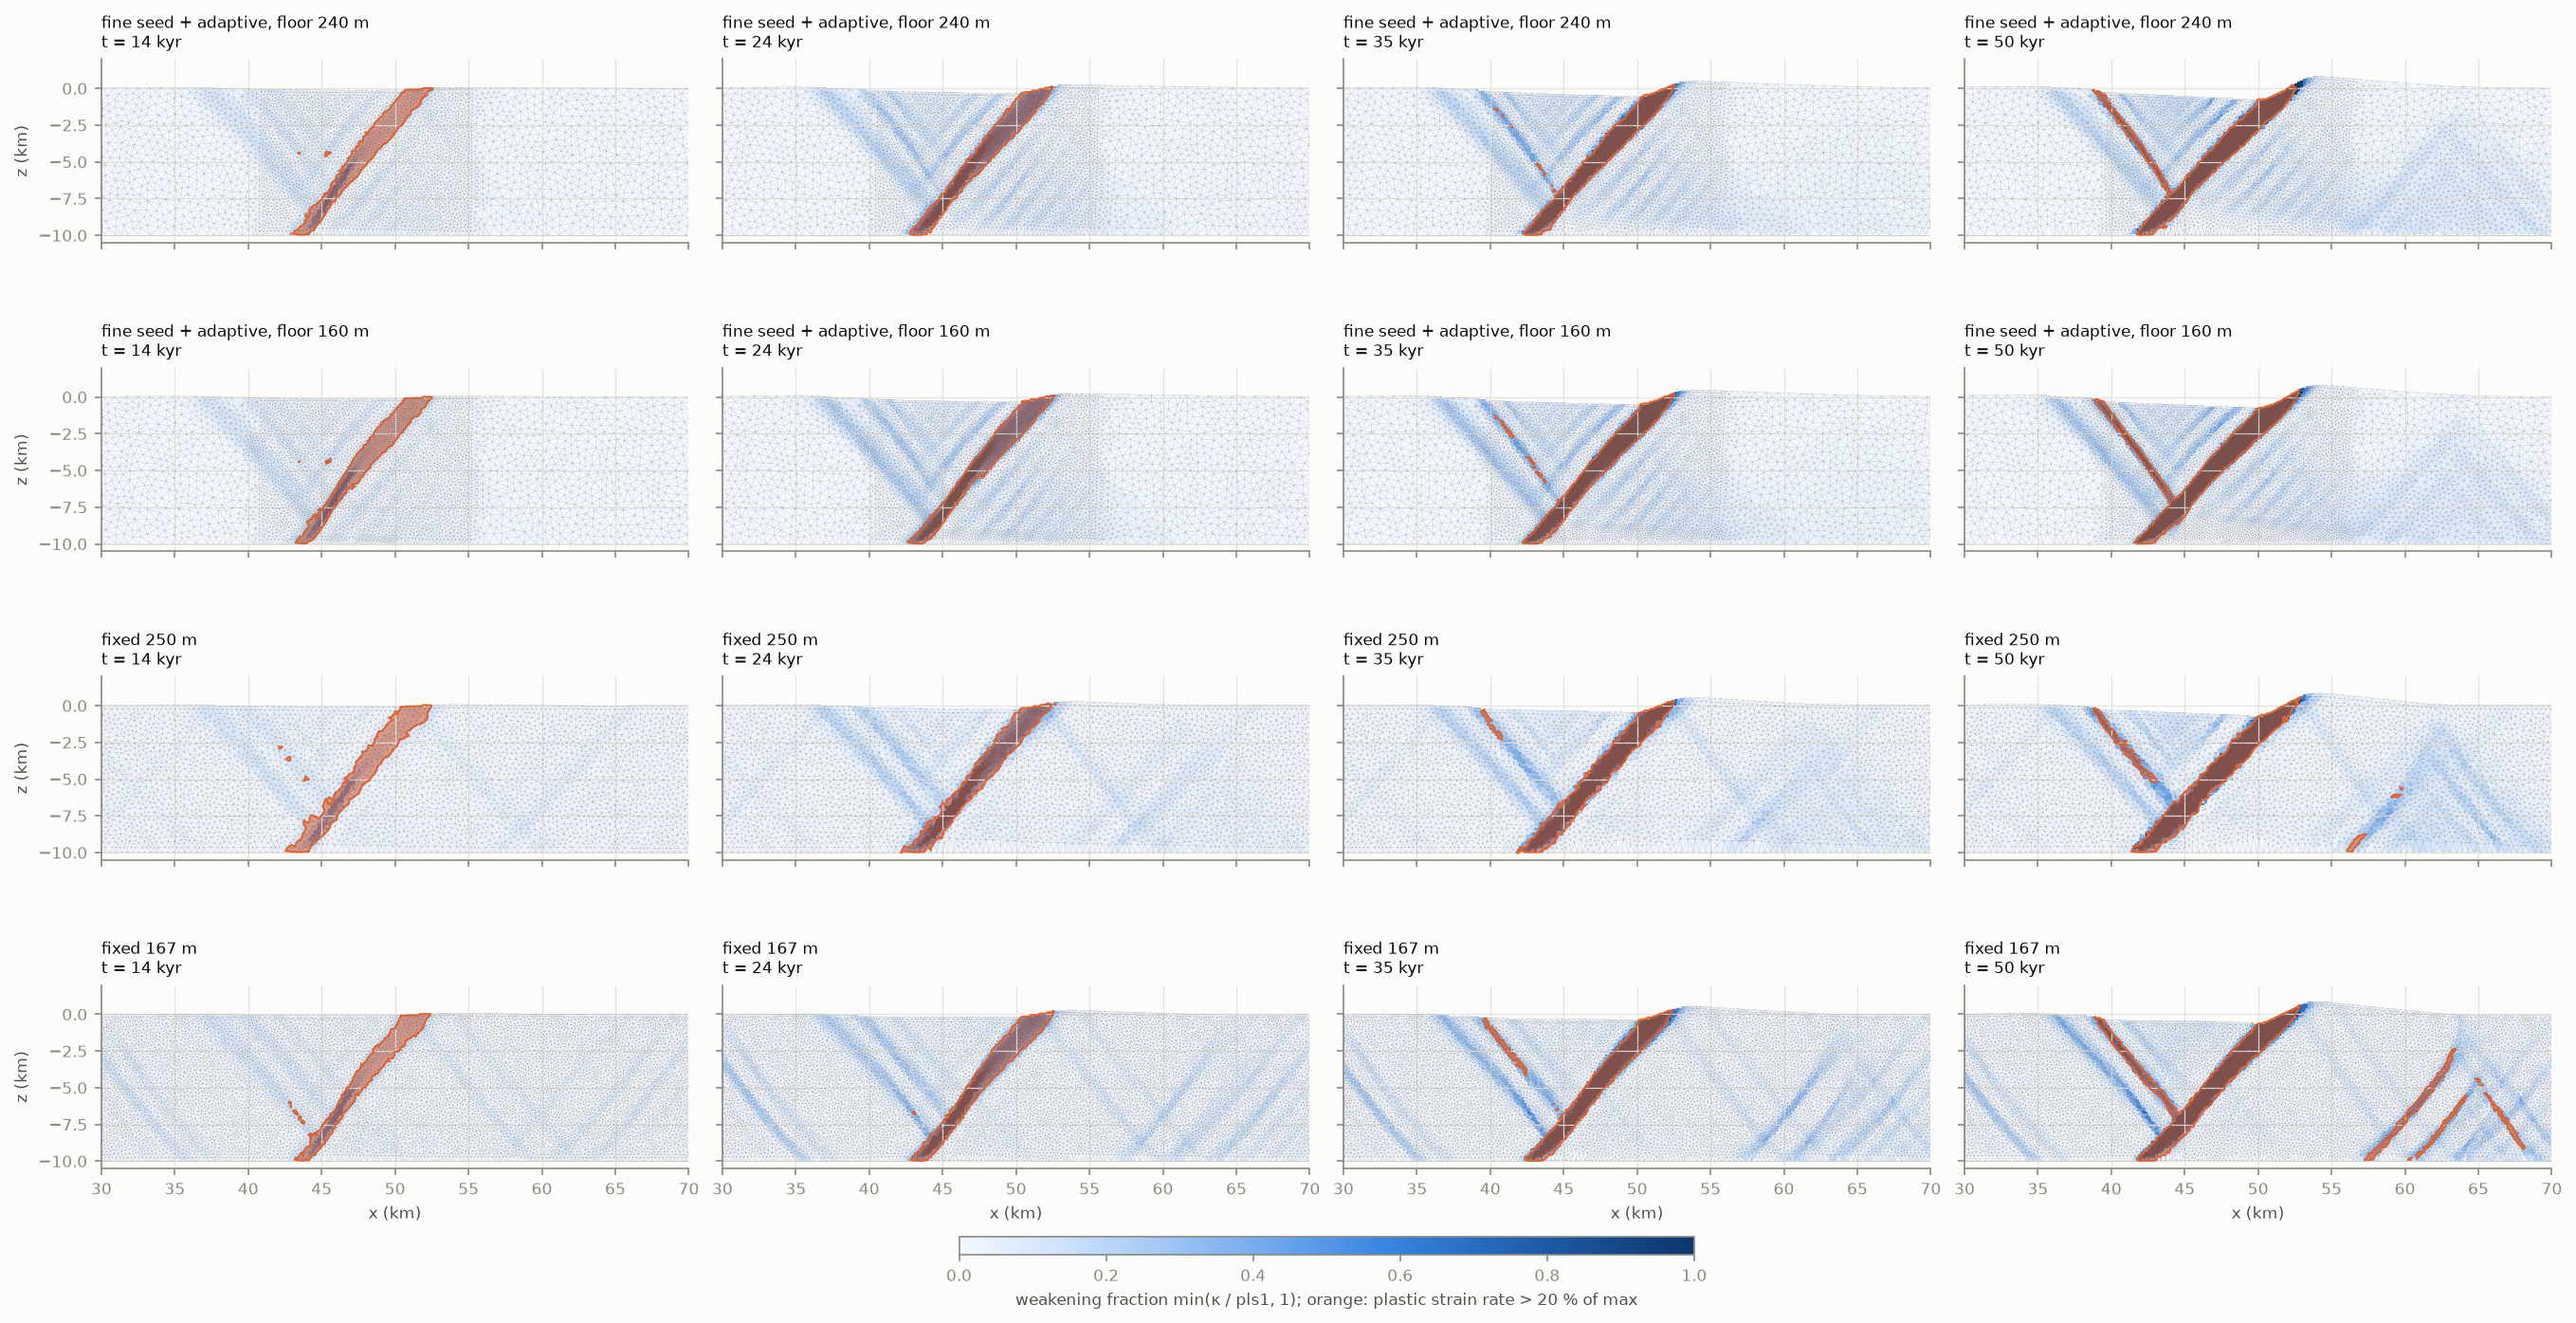
\includegraphics[width=\textwidth]{fig_seed_maps.png}
  \caption{$\tau=3.3\times10^8$\,s at 14, 24, 35 and 50\,kyr. Rows: fine seed + adaptive mesh with a
  240\,m floor (the example), the same with a 160\,m floor, fixed 250\,m, fixed 167\,m. Colours as in
  Fig.~\ref{fig:taumaps}; the mesh is drawn in grey. The main fault and the hanging-wall fault are the
  same in all four. The faults at $x\approx58$--68\,km that form in the fixed 167\,m run by 50\,kyr
  do not form in the adaptive runs: they start outside the refined zone, on coarse elements.}
  \label{fig:seedmaps}
\end{figure}

\begin{figure}[p]
  \centering
  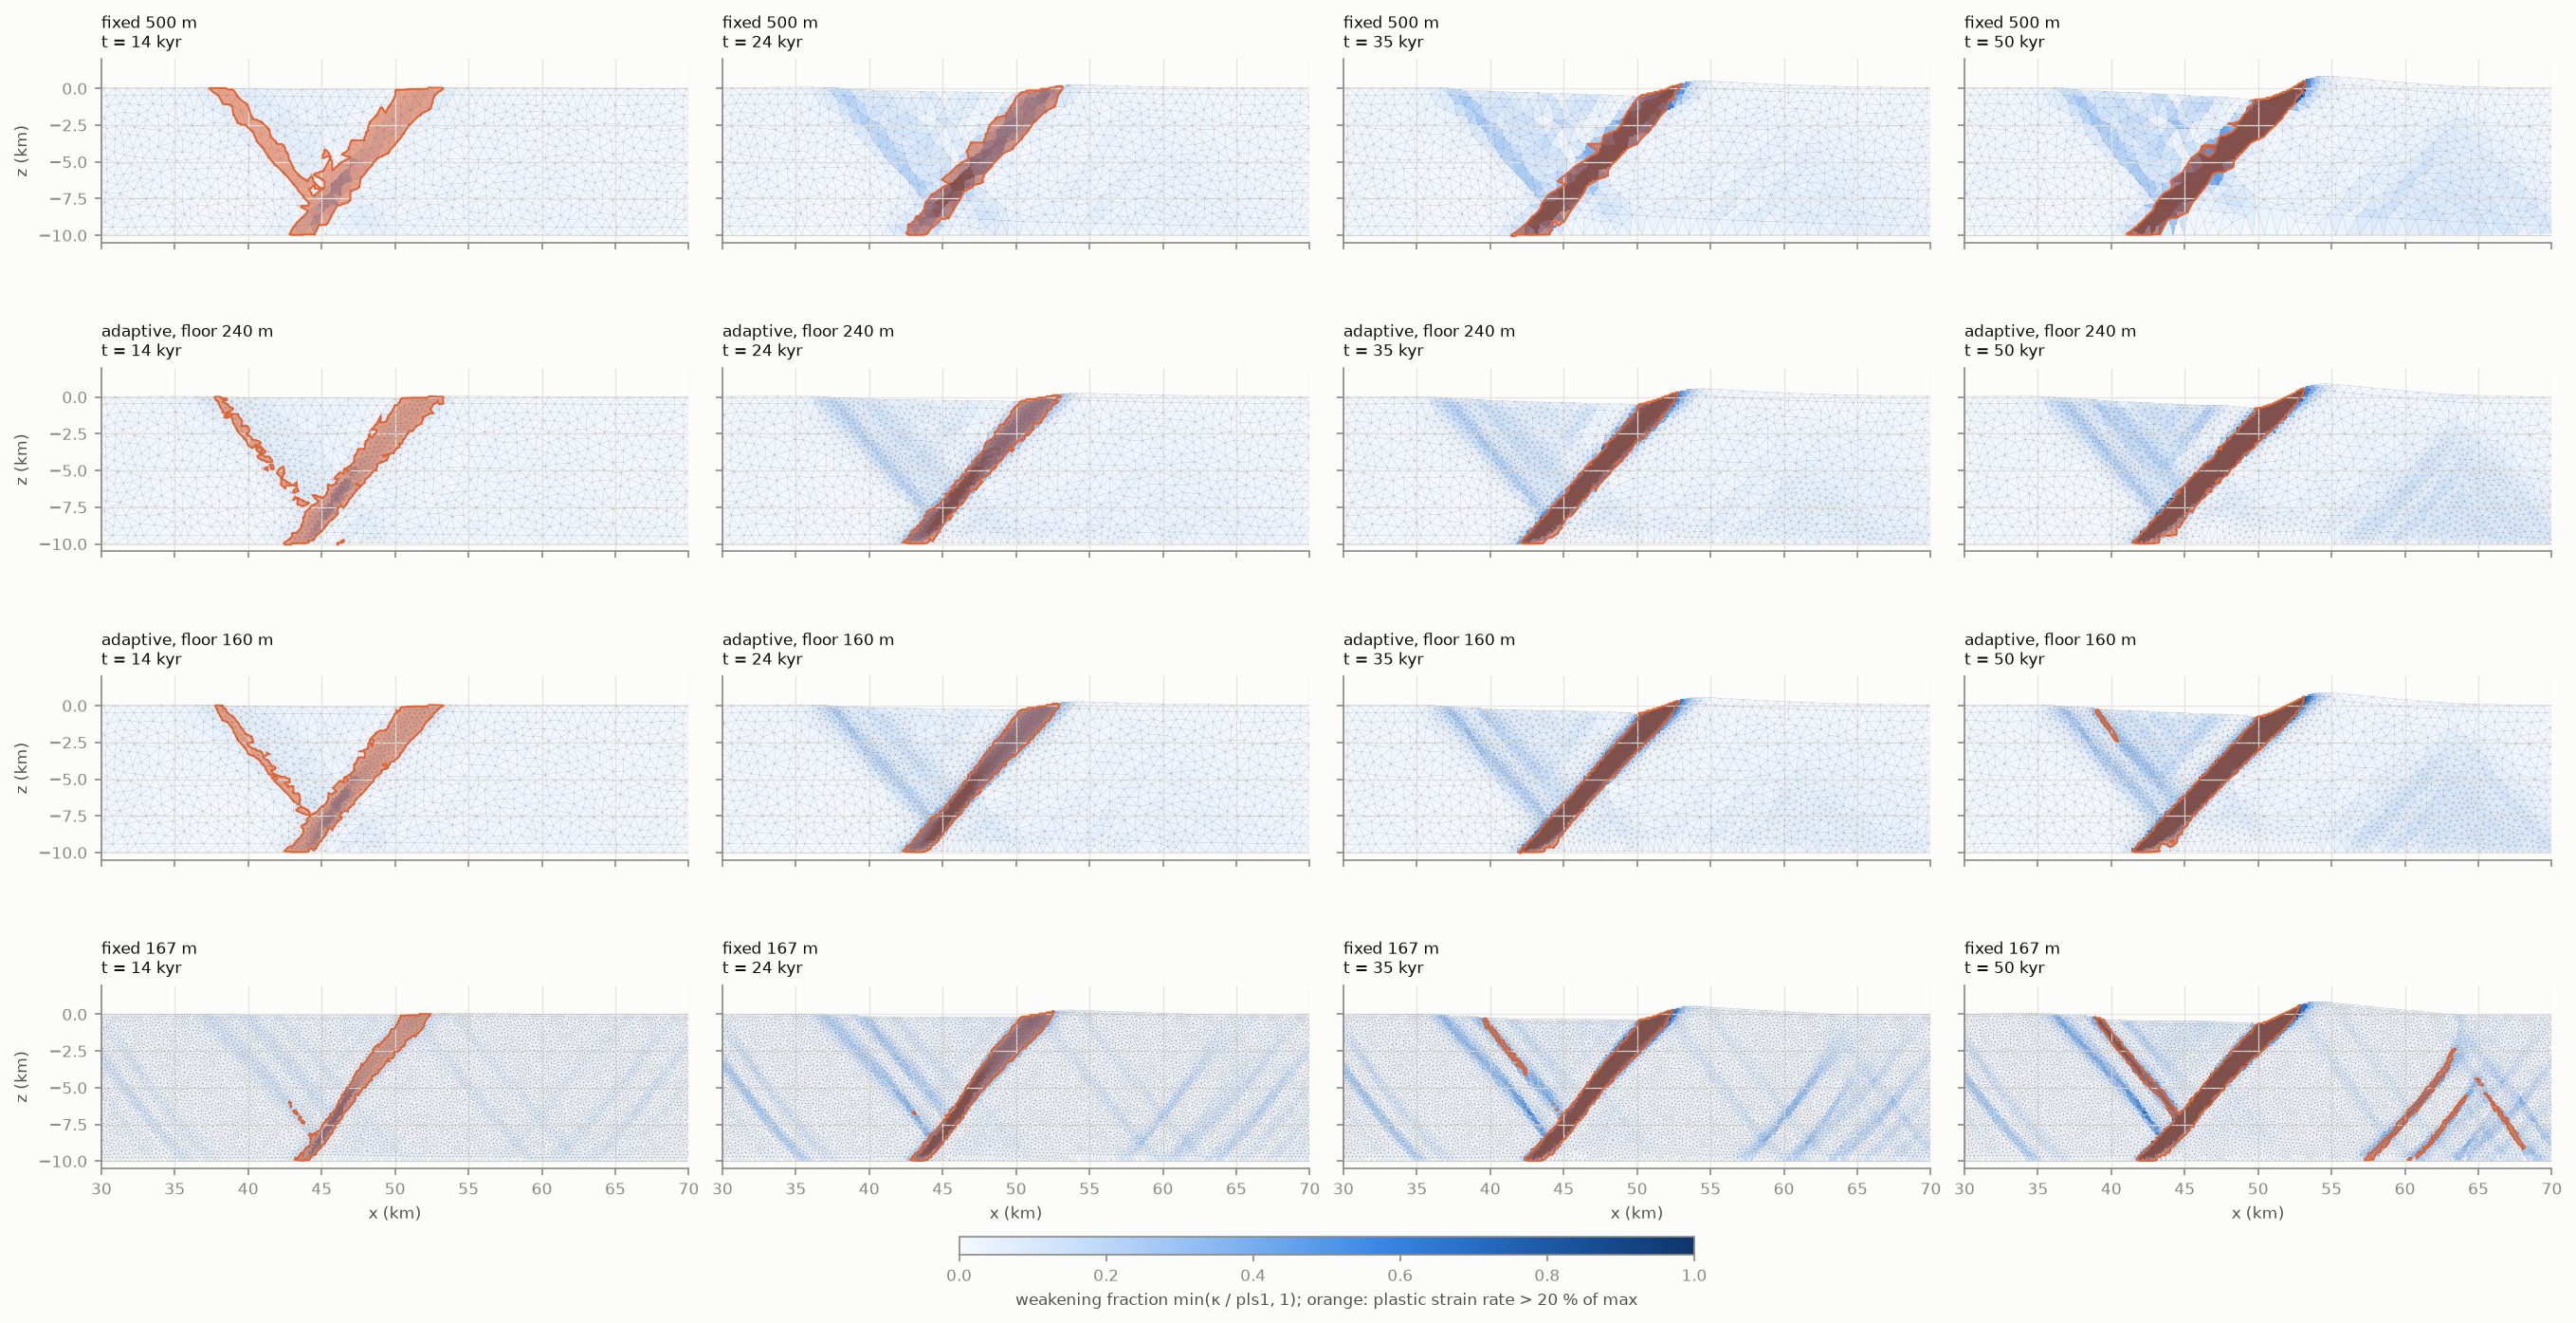
\includegraphics[width=\textwidth]{fig_amr_maps.png}
  \caption{$\tau=3.3\times10^8$\,s, starting from a \emph{coarse} seed on 500\,m elements. Rows:
  fixed 500\,m; 500\,m with MMG refinement, floor 240\,m; same with floor 160\,m; fixed 167\,m for
  reference. On the coarse start a conjugate pair forms at 14\,kyr; the band forms on 500\,m elements
  before the first remesh (8.9\,kyr) and, once refined, keeps a width $\approx15$\,\% larger than the
  fine-start runs (Table~\ref{tab:amr}).}
  \label{fig:amrmaps}
\end{figure}

\paragraph{Reading Table~\ref{tab:amr}.} Stopping the refinement at $\approx W/5$ is enough: the 240
and 160\,m floors differ by 3\,\% late in the run, and both are within 2--5\,\% of the fixed meshes,
with half the elements of the fixed 167\,m mesh. The band must, however, \emph{start} on fine
elements: a band that forms on coarse elements keeps its coarse width after refinement.

%======================================================================
\section{Duvaut--Lions with high-pass damping}
\label{sec:damping}

The two address different problems. Duvaut--Lions fixes \emph{where} and \emph{how wide}
deformation localizes; high-pass mass damping (\code{control.has\_highpass\_damping}, companion
note) removes the pseudo-elastic waves of the mass-scaled solver, which produce strain-rate noise
but not the band width. Their time scales are separated in the core complex: the damping acts on
fluctuations faster than $T_f=10^{10}$\,s and decays them over $1/\alpha=2\times10^7$\,s, while
$\tau=3.3\times10^8$\,s.

\paragraph{Test.} \code{examples/core-complex-dl.cfg} as committed ($\tau=3.333\times10^8$\,s, thin
seed, refined zone $x=41$--55\,km, MMG refinement with a 240\,m floor, 50\,kyr, output averaging
off), run twice with the branch head (\code{8ea5a49}): Duvaut--Lions alone, and Duvaut--Lions with
high-pass damping at the defaults ($\alpha=5\times10^{-8}$\,s$^{-1}$, $T_f=10^{10}$\,s). Metrics as
in the companion note; the band width is $\int\dot\varepsilon_p\,dx/\max\dot\varepsilon_p$ over
$x_f\pm2$\,km at $z=3,5,7$\,km, with the main fault $x_f$ located at 50\,kyr. This fixed corridor
differs from the band tracking of Sect.~\ref{sec:conv}, so the widths are comparable between the
two runs here, not one-to-one with Table~\ref{tab:amr}. Both runs took $\approx37$\,min on 4
threads and ended with $\approx13\,600$ elements.

\begin{table}[h]
  \centering\small
  \caption{\code{core-complex-dl.cfg}, Duvaut--Lions alone (DL) vs with high-pass damping (+d).
  Per window: slip-rate jump, plastic-integral jump, mean slip rate, main-fault width, background
  p10 of $\log_{10}\dot\varepsilon_{II}$.}
  \label{tab:dlhp}
  \setlength{\tabcolsep}{4pt}
  \begin{tabular}{lcccccccccc}
  \toprule
  window & \multicolumn{2}{c}{jump slip} & \multicolumn{2}{c}{jump plastic} & \multicolumn{2}{c}{slip ($10^{-9}$\,m/s)} & \multicolumn{2}{c}{width (km)} & \multicolumn{2}{c}{bg p10}\\
  (kyr) & DL & +d & DL & +d & DL & +d & DL & +d & DL & +d\\
  \midrule
  5--15  & 0.086 & 0.053 & 0.002 & 0.003 & 1.26 & 1.15 & 1.42 & 1.32 & $-15.1$ & $-15.6$\\
  15--25 & 0.010 & 0.009 & 0.017 & 0.005 & 1.81 & 1.78 & 1.19 & 1.18 & $-15.2$ & $-15.7$\\
  25--35 & 0.047 & 0.021 & 0.038 & 0.006 & 2.08 & 2.10 & 1.22 & 1.22 & $-14.8$ & $-15.9$\\
  35--42 & 0.010 & 0.002 & 0.003 & 0.007 & 1.91 & 1.91 & 1.38 & 1.41 & $-14.9$ & $-16.0$\\
  42--50 & 0.186 & 0.016 & 0.065 & 0.007 & 1.64 & 1.76 & 1.48 & 1.47 & $-14.5$ & $-15.9$\\
  \bottomrule
  \end{tabular}
\end{table}

\begin{figure}[H]
  \centering
  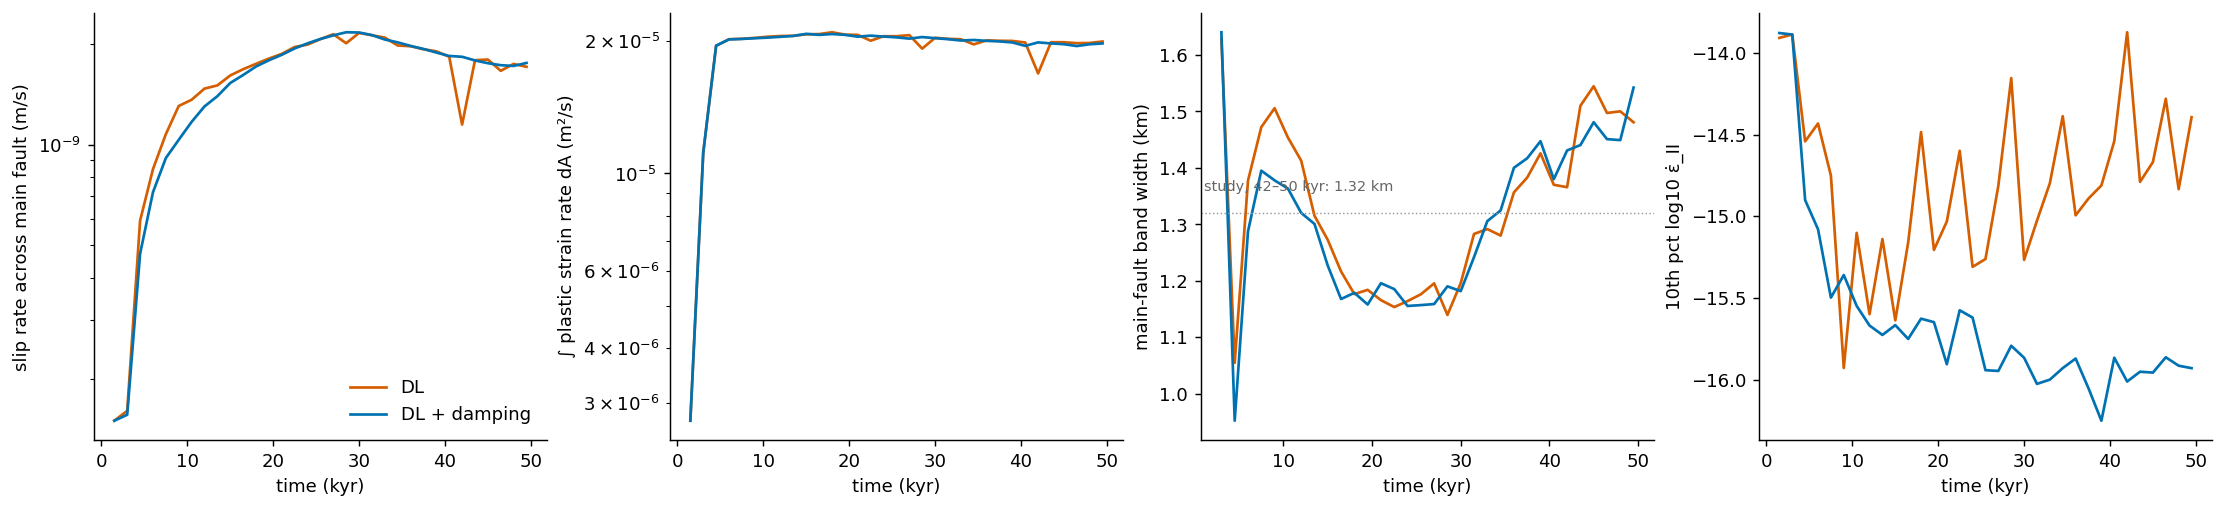
\includegraphics[width=\textwidth]{fig_dl_series.png}
  \caption{\code{core-complex-dl.cfg}: Duvaut--Lions alone (orange) and with high-pass damping
  (blue). Left to right: slip rate across the main fault, plastic-strain-rate integral, main-fault
  band width, 10th percentile of $\log_{10}\dot\varepsilon_{II}$. Slip rate, plastic integral and
  width coincide; the slip dip at 42\,kyr and the background noise (right) are removed by the
  damping. Dotted: the 42--50\,kyr width of the example in Table~\ref{tab:amr}.}
  \label{fig:dlseries}
\end{figure}

\begin{figure}[p]
  \centering
  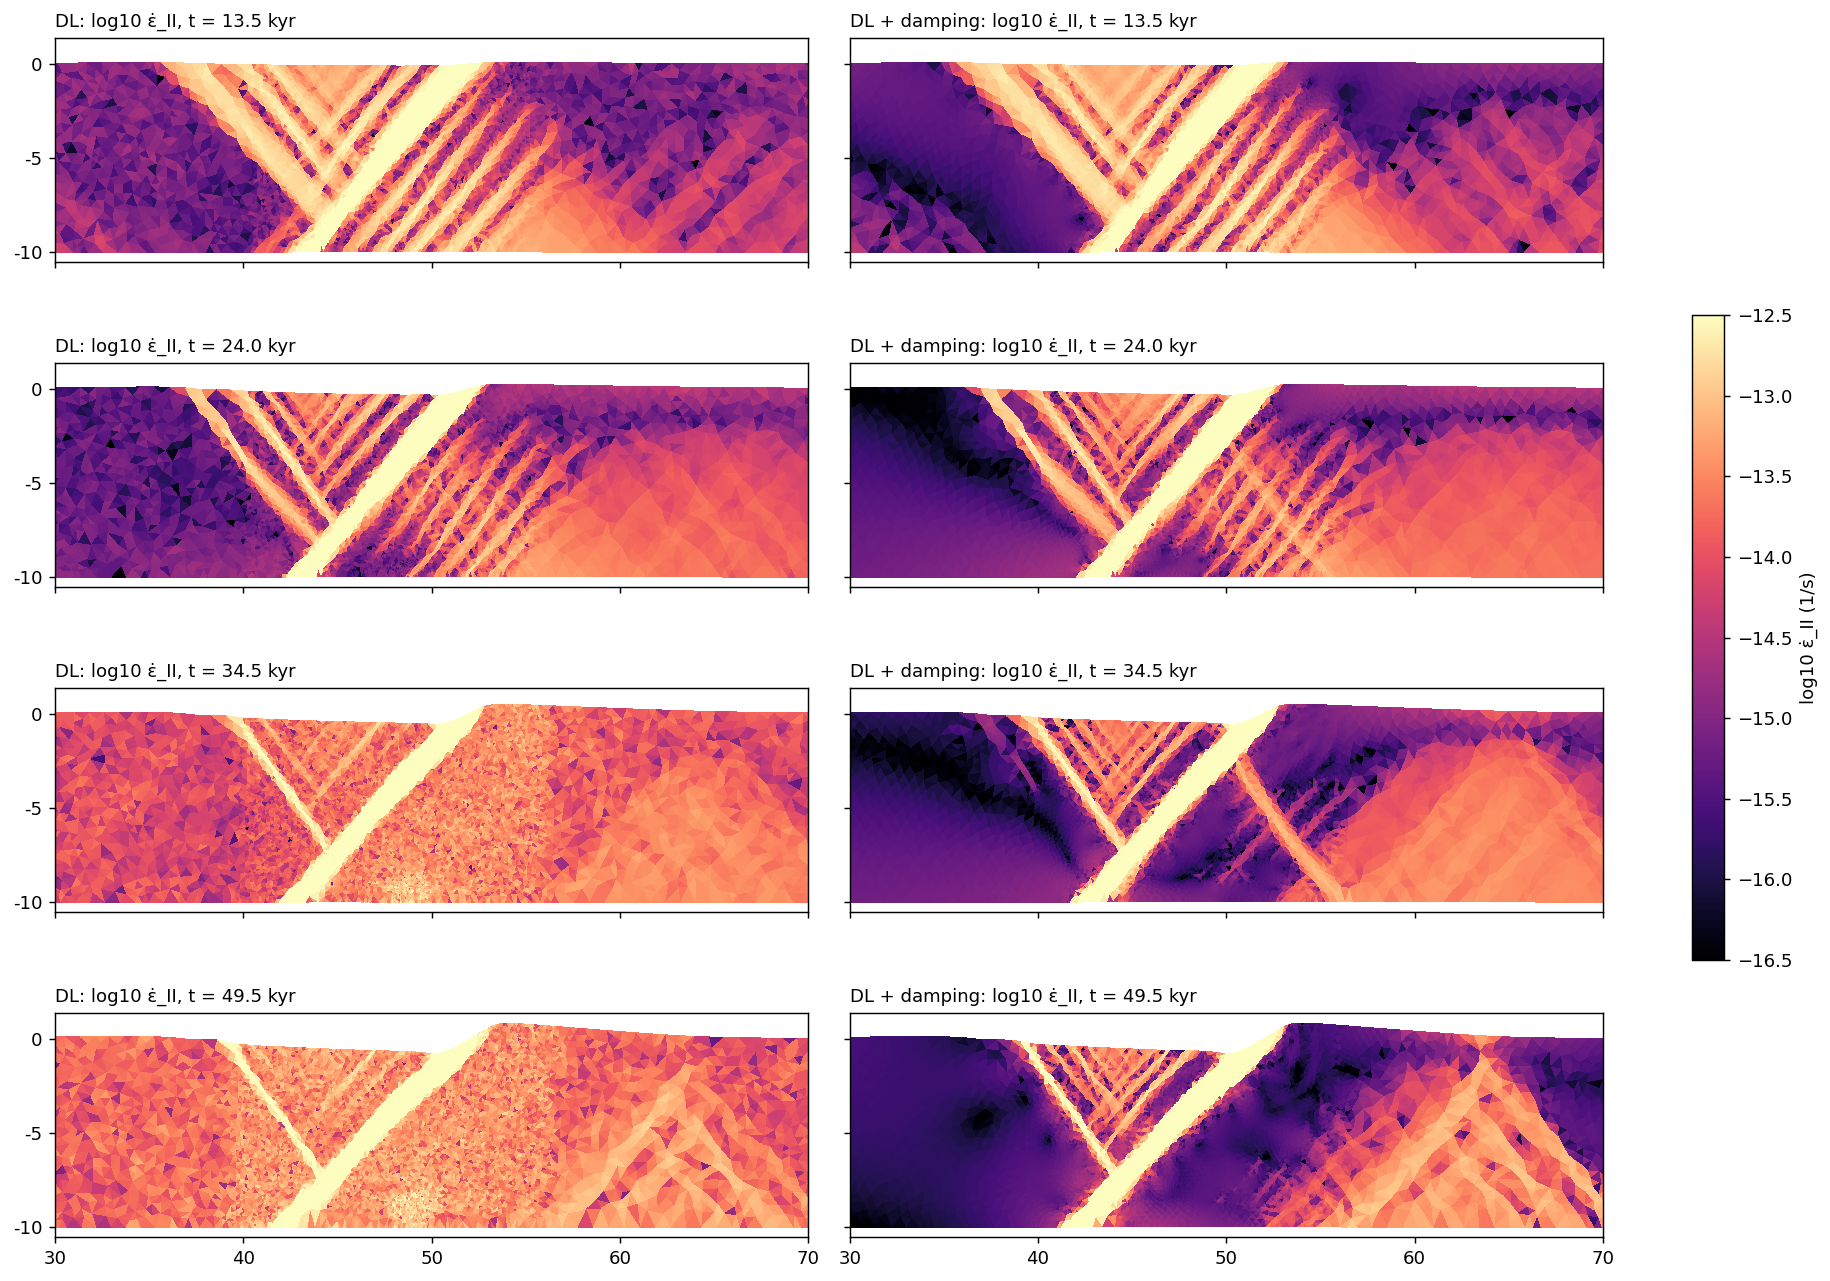
\includegraphics[width=\textwidth]{fig_dl_sr.png}
  \caption{$\log_{10}\dot\varepsilon_{II}$ at 13.5, 24, 34.5 and 49.5\,kyr; Duvaut--Lions alone
  (left) and with damping (right); instantaneous fields; $x=30$--70\,km. With Duvaut--Lions alone the
  band structure is clean early, but by 34.5 and 49.5\,kyr the hanging wall and footwall are filled
  with element-scale noise at $\sim10^{-13.5}$\,s$^{-1}$, as in the rate-independent code. With
  damping the background stays at $10^{-15.5}$--$10^{-16}$\,s$^{-1}$ and the main fault, its
  hanging-wall conjugates and the footwall bands are all distinct.}
  \label{fig:dlsr}
\end{figure}

\begin{figure}[p]
  \centering
  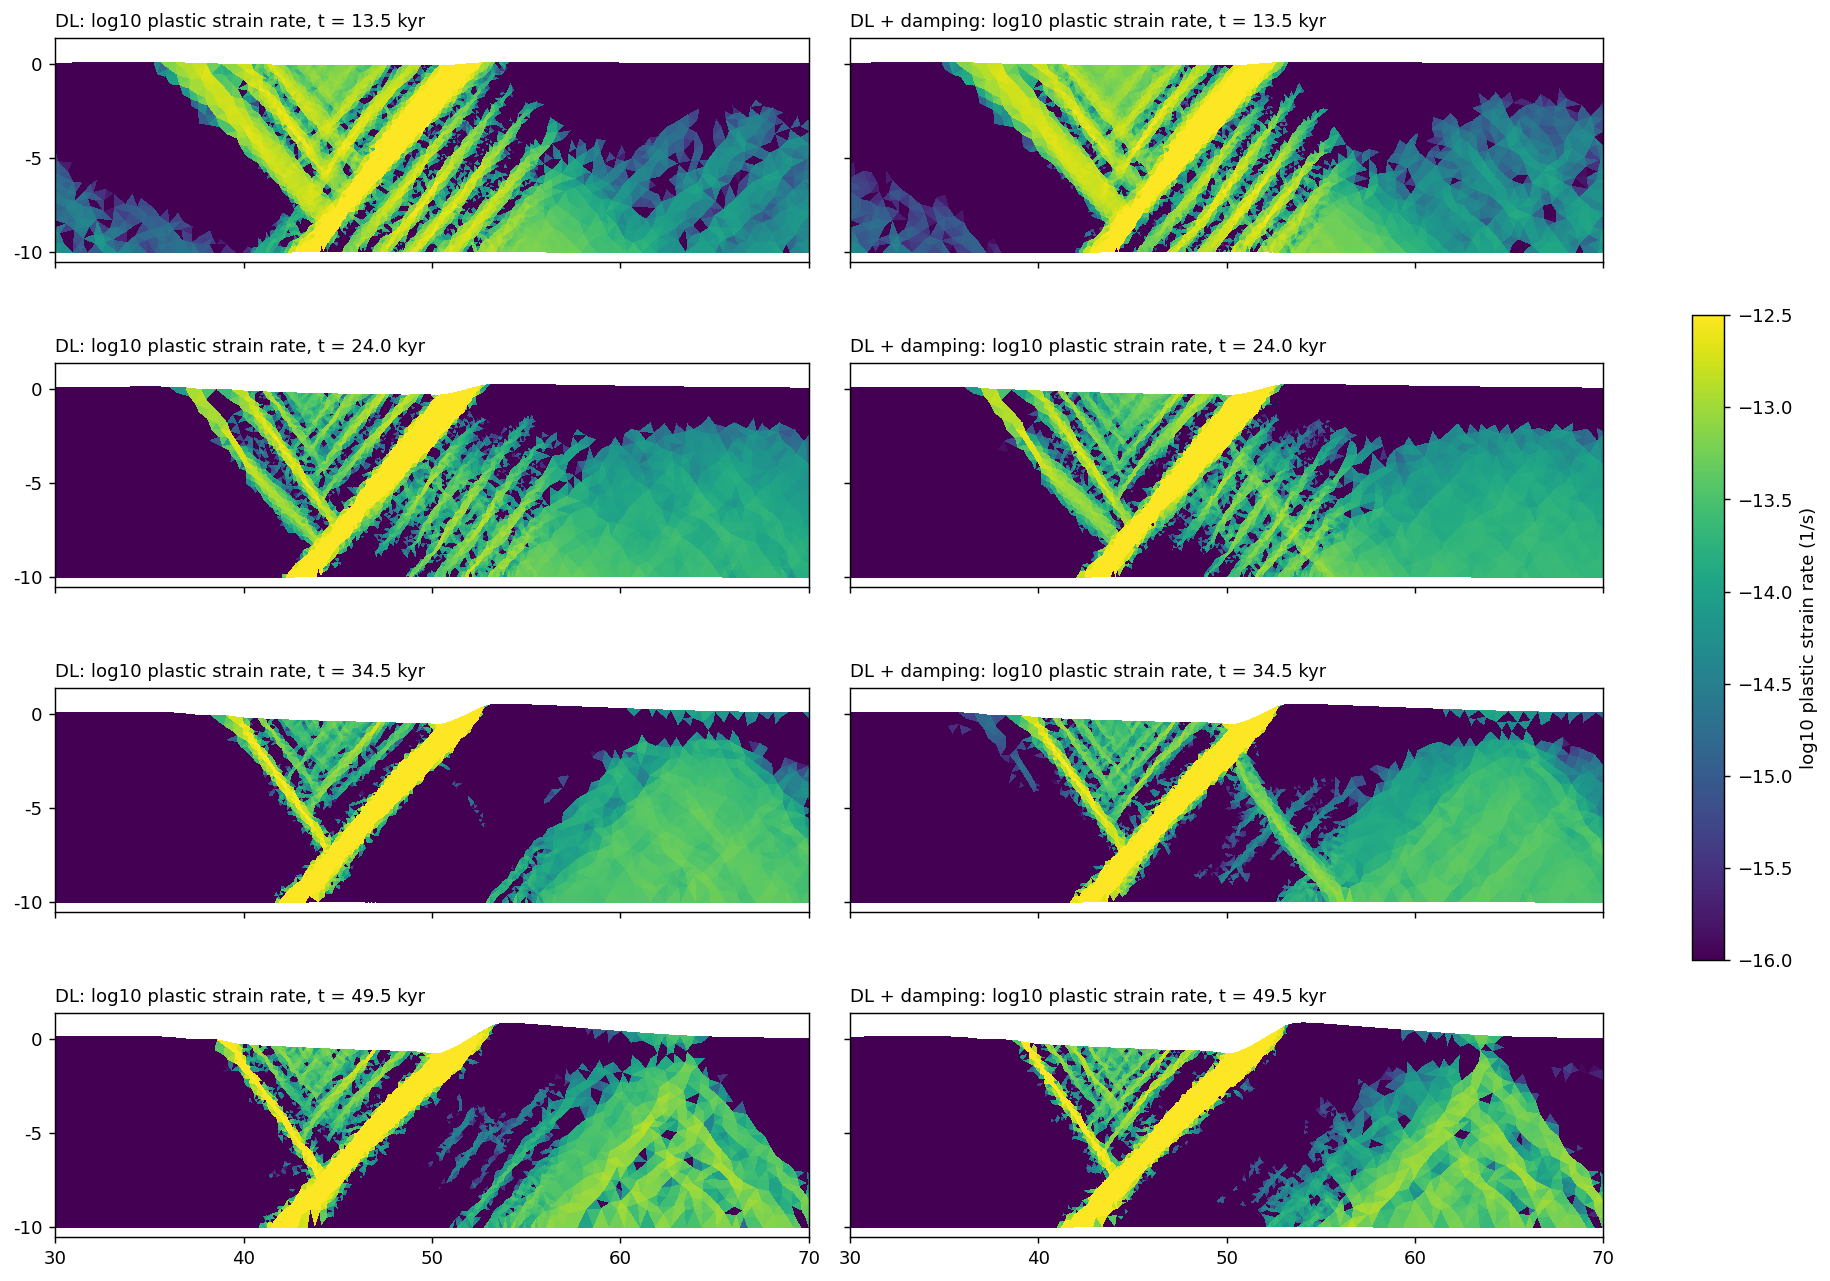
\includegraphics[width=\textwidth]{fig_dl_pl.png}
  \caption{$\log_{10}$ plastic strain rate for the same runs and times (per-step output divided by
  $\Delta t$). The active main fault and the hanging-wall conjugate set are the same in both. At
  34.5\,kyr the damped run has an active conjugate band crossing the dome ($x\approx52$--57\,km) that
  is not active in the undamped run at that frame; by 49.5\,kyr the patterns are again alike. The
  broad region of low-level yielding in the footwall ($x>55$\,km) is present in both.}
  \label{fig:dlpl}
\end{figure}

\paragraph{Results.}
\begin{itemize}
\item \emph{The damping does not change the regularized fault.} Fault position within 0.3\,km at
  every depth (48.4/46.6/45.3 against 48.7/46.4/45.0\,km at $z=3/5/7$\,km); widths within 0.1\,km
  in every window and within 0.03\,km after 15\,kyr; median difference of the slip rate 1.9\,\% and of
  the plastic integral 0.5\,\%; same element count and run time.
\item \emph{Duvaut--Lions alone is already much quieter than the rate-independent code.} Its
  slip-rate jump is 0.01--0.09 in most windows, against 0.44 for the rate-independent original at
  167\,m over 15--30\,kyr (companion note; same seed, but a fixed mesh). This supports the expectation
  of Fig.~\ref{fig:element}C that spreading each stress drop over $\tau$ radiates less wave noise.
\item \emph{But not quiet enough on its own.} The background strain rate fills with element-scale
  noise as the model evolves (p10 rising from $-15.1$ to $-14.5$; Fig.~\ref{fig:dlsr}), and at
  42\,kyr the slip rate dips by $\approx35$\,\% within one frame (slip jump 0.19 at 42--50\,kyr). With
  damping the background stays about one order of magnitude lower ($-15.6$ to $-16.0$), the dip is
  gone (jump 0.016), and the plastic-integral jump falls three- to nine-fold in the windows after
  15\,kyr, except 35--42\,kyr where both are already below 0.01.
\item \emph{One transient difference}: an active conjugate across the dome at 34.5\,kyr in the damped
  run only (Fig.~\ref{fig:dlpl}). Single runs cannot tell whether this is an effect of the damping or
  of the sensitivity of secondary faulting to small differences.
\end{itemize}
The two methods therefore combine without side effects on the regularized fault, and each does what
the other cannot: Duvaut--Lions sets the band width, the damping removes the noise that remains.
This is one case (2D, one $\tau$, one mesh strategy).

%======================================================================
\section{Limitations}
\label{sec:lim}

\paragraph{Resolution.} The width becomes mesh independent only when about five elements span it.
For $W\approx1$\,km that means $\approx200$\,m elements wherever a fault can form; on the core complex
only $\tau=3.3\times10^8$\,s converged at 250--167\,m, and only after $\sim40$\,kyr. Smaller $\tau$
(narrower, more realistic bands) need proportionally finer meshes. A regularized model is not
cheaper than the original; it is convergent.

\paragraph{Faults outside the refined zone.} MMG refinement on plastic strain acts only after
plastic strain has built up, so a fault that starts on coarse elements forms late or not at all: the
faults at $x\approx58$--68\,km that appear in the fixed 167\,m run do not form in the adaptive runs by
50\,kyr (Fig.~\ref{fig:seedmaps}). The refined zone must cover every place a fault may start. A metric
driven by the plastic strain \emph{rate} might remove this; it has not been tried.

\paragraph{Seeds and refined-zone edges.} A seed wider than $W$ and already softened imposes its own
width (Sect.~\ref{sec:conv}); the edge of a refined zone can nucleate faults (Fig.~\ref{fig:zone}).
Both must be designed with $W$ in mind. \code{examples/core-complex.cfg} has been left unchanged:
switching it to the thin seed and the wider zone would change the benchmark's results.

\paragraph{$\tau$ is physics, not only numerics.} The overstress adds up to $G\tau\dot\kappa$ to the
fault strength --- 12--19\,MPa for $\tau=3.3\times10^8$\,s against a residual cohesion of 4\,MPa. The
regularized fault is rate strengthening with $\eta_{vp}=10^{19}$\,Pa\,s. Choosing $\tau$ to obtain a
convenient width therefore also chooses a fault rheology; results that depend on fault strength
(stress drops, the competition between faults, the brittle--ductile transition) depend on $\tau$.
In \code{rh\_evp} the overstress raises the plastic candidate, so the viscous candidate wins more
often than without regularization; this shift has not been quantified.

\paragraph{Calibration.} The width estimate (Eq.~\ref{eq:width}) and the 3--5-element rule were
calibrated on one setup (2D core complex, one material, \code{pls1} = 0.5, dilation 0). Other
softening laws, dilatancy, 3D and multi-material models have not been tested for convergence; in 3D
only the regression check ($\tau=10^{10}$\,s changes results) was run.

\paragraph{Rheologies and platforms.} Only \code{rh\_ep} and the plastic candidate of \code{rh\_evp}
are regularized; rate-and-state rheologies are rejected. The helper is compiled for OpenACC, but GPU
runs were not part of this study.

\paragraph{Reproducibility of this note.} The figures and tables of Sects.~\ref{sec:conv}--\ref{sec:recipe}
come from the issue \#109 study. The scripts are in \code{regularization/nonlocal-figures/scripts/},
but the run outputs they read were not preserved, so those figures cannot be regenerated without
rerunning the models; the width table (\code{thin-seed/main\_fault.csv}) is kept. The runs of
Sect.~\ref{sec:damping} are in \code{highpass-runs/dl2-off} and \code{dl2-on}, analysed by
\code{cmp\_dl.py}. With output averaging off, DES writes ``plastic strain-rate'' as the per-step
increment; \code{cmp\_dl.py} divides it by $\Delta t$. The width measure of the \#109 study is a ratio
and is not affected.

\paragraph{Status.} The option is on the unmerged branch \code{feat/regularization} (commits
\code{40ccbba}, \code{ff3415b}), proposed in issue \#109.

%======================================================================
\section{Summary}
\begin{itemize}
\item Duvaut--Lions blends the elastic trial stress with the rate-independent return,
  $\sig=(1-w)\sig^{tr}+w\sig^{RI}$ with $w=\Delta t/(\tau+\Delta t)$, and scales the plastic-strain
  increment by $w$. It reuses the existing return map and is bit-identical at $\tau=0$.
\item It makes plastic flow rate strengthening with $\eta_{vp}=G\tau$, which gives shear bands a width
  $W\approx2.3\,G\tau V/\Delta c$ (prefactor measured on the core complex); the measured overstress follows $G\tau V/W$ with one constant across
  $\tau$ and meshes.
\item On the core complex with a thin seed and a wide refined zone, $\tau=3.3\times10^8$\,s gives a
  mesh-independent main fault (1.34 and 1.35\,km at 250 and 167\,m) and keeps the core-complex
  geometry, once about five elements span the band.
\item With high-pass damping added, the regularized fault is unchanged (position within 0.3\,km,
  width within 0.03\,km after 15\,kyr, slip rate within 2\,\%), and the background noise and slip-rate
  bursts that Duvaut--Lions leaves are removed.
\item Choose $\tau$ from the target width, give every place a fault may start elements of $W/5$, and
  stop refining there. The cost: resolution where faults can form, and a rate-strengthening fault
  rheology that is part of the physics.
\end{itemize}

\end{document}
